%!TEX root = ../konzept.tex

\section{Benutzermodellierung}
%Wer sind die Benutzer

TODO textliche Einführung

\begin{figure}[H]
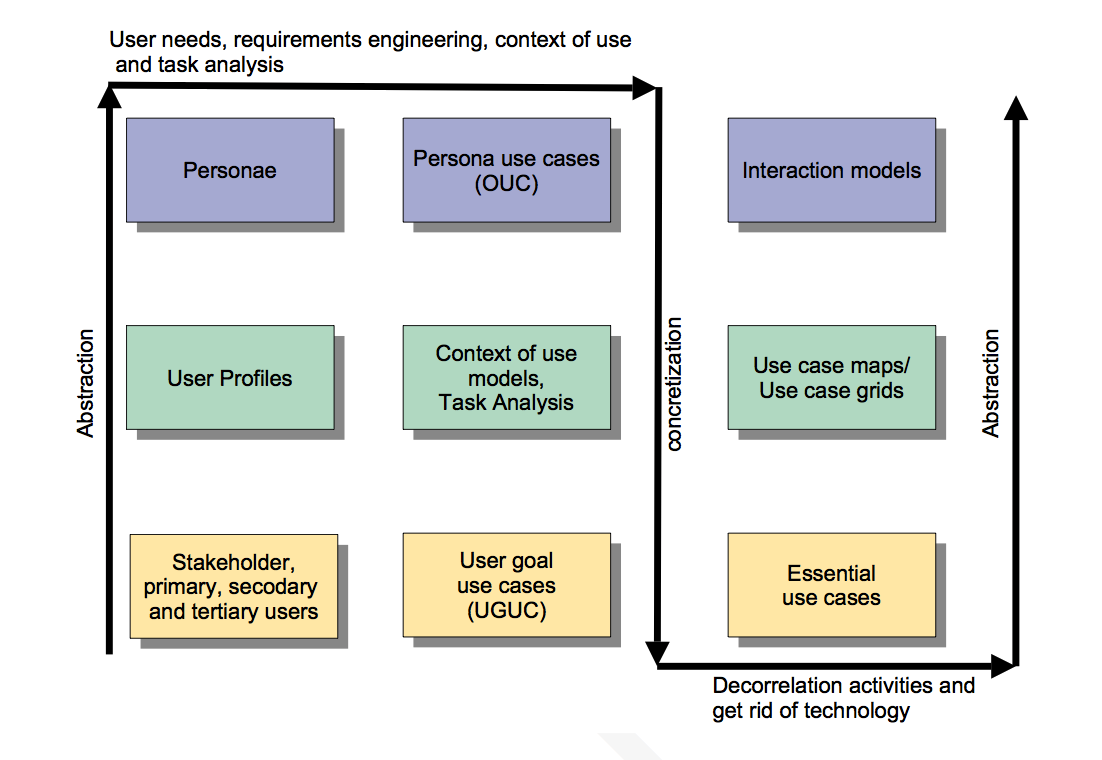
\includegraphics[width=.9\textwidth]{./images/benutzermodellierung.png}
\caption{Prozessmodell benutzerzentrierten Vorgehens}
\label{prozessmodell}
\end{figure}

\subsection{Stakeholderanalyse}
Die erste Stufe der Benutzermodellierung dient der Identifikation potentieller Nutzergruppen des Systems.
Das Spektrum an Interessenten und Betroffenen innerhalb der Anwendungsdomäne, wird dazu in
verschiedene Benutzerklassen eingeteilt.\\
 
Als primary User des Systems, letztendlich die Enduser, die direkt mit der Anwendung interagieren, wurden folgende Benutzer ermittelt:
 
Zum einen wird die Anwendung von Interessenten in der Tätigkeit des Mietenden verwendet.
Diese können grundsätzlich aus allen Altersgruppen stammen, vorausgesetzt sie sind voll geschäftsfähig, da ein Mietgeschäft stattfindet, und sie sind im Besitz der benötigten Hardware.
Eingrenzen lässt sich das Benutzerfeld weiterhin auf Reisende oder Touristen, die eine Unterkunft benötigen und im Regelfall Campingausrüstung bei sich tragen. In diese Kategorie fallen demnach auch Personen wie Backpacker, Langzeitreisende, Wanderer.
Sie suchen entweder aktiv selbst oder sind diejenigen, die mit der Funktionalität im späteren Verlauf, beispielsweise bei einem QR Code check, direkt in Kontakt mit der Anwendung kommen.
 
Die zweite Interessentengruppe sind die Vermieter, die ihr Grundstück als Unterkunft zur Verfügung stellen. Auch hier wirkt vorherige Einstufung der Altersgruppe, wobei die Verfügbarkeit der Hardware in der Regel zu einer gewissen Altersgrenze führen wird, die Schätzungsweise bis 50 Jahre geht. (Hierbei könnte man sich auf Statistiken berufen. Vorerst Schätzwert)
Vermieter in der Rolle des primary users sind Grundstücksbesitzer bzw. Garteneigentümer und Personen, welche während des Mietprozesses aktiv mit der Anwendung interagieren.\\
 
Weitere Betrachtung widmet sich den secondary usern, welche nicht regelmäßig selbst mit der Applikation interagieren. Sie liefern den primary usern entsprechenden Input, diese benutzen die Anwendung dann an ihrer Stelle als Zwischennutzer und geben den erhaltenen Output zurück. Für diese Benutzergruppe wurde auf Mieterseite die „erweiterte“ Reisegruppe definiert. Jeder der neben dem eigentlichen Benutzer die Unterkunft benutzt und im Vorfeld aktiv an der Suche beteiligt ist, indem beispielsweise Anhaltspunkte gegeben werden in welchem Umkreis gesucht werden soll.
Für den Vermieter ergibt sich hierbei der Personenkreis, der selbst ein Grundstück zur Verfügung stellen kann und möchte, aber entsprechende Technologien nicht besitzt und das Angebot jemand anderen Abwickeln lässt. Die Anzahl dieser Anwendertypen wird im Vergleich zu den vorherigen Benutzergruppen jedoch eher gering eingeschätzt.\\
 
Als weitere Stakeholder im Bereich der Entscheidungsträger für spätere Anschaffung und Benutzung (tertiary user) wurden potentielle Werbepartner identifiziert, die als Teil des Geschäftsmodells zum Beispiel bei Events auftreten können. Zusätzlichen Einfluss kann die Anwendung außerdem auf die Stadt in Form von Tourismus haben und dabei auch mit bestehenden Unterkunftsanbietern wie Hotels, Hostels oder öffentlichen Campingplätzen konkurrieren. Auch wenn diese nicht zwangsläufig als Nutzer der Anwendung auftreten, so haben sie Interesse am möglichen Erfolg und Misserfolg und können dementsprechend beeinflusst werden.
Dazu kommen Personen aus organisatorischen Bereichen wie System Administratoren oder Supportmitarbeiter.\\
 
Für die spätere Auseinandersetzung ist es notwendig die wichtigsten Stakeholdergruppen zu bestimmen und dahingehend die Anforderungsermittlung durchzuführen.
In Anbetracht des Projektziels fallen hierbei vorerst die primary und secondary user auf, die in einer detaillierten Auseinandersetzung innerhalb der User Profiles genauer bestimmt werden sollen.
 
Da die menschzentrierte Entwicklung ein iterativer Prozess ist, kann zu späteren momenten eine erneute Auseinandersetzung mit den gewonnen Erkenntnissen stattfinden.
Ansätze hierbei wäre ein Perspektivwechsel nach Tätigkeitsperspektive, Rollenperspektive, Interessenperspektive pderkulturelle Perspektive sowie Ergebnisse aus weiterer Marktanalyse und Recherche, eventuell auch unter Einbezug möglicher Interessenten. (Interviews etc.)
 

 \subsection{User Profiles}

- detaillierte Stakeholder
- sinnvolle Merkmale
- demographisch: Alter, Wohnort?
- Erfahrung mit Smartphones/Applikationen
- Berufserfahrung: für Anwendung irrelevant
- Fachwissen: Erfahrung als Reisender/ Camper
- physiologische Eigenschaften:
- Aufgaben
- verfügbare Technologien
- kultureller Hintergrund: Sprache
- spezielle Produkterfahrung: domain spezifische Konkurrenz?
- Motivation
- Einstellung/Werte:  Produkt Preferenzen, Technologieängste
 
- sachliche Darstellung, Tabellenform, Reduktion aufs wesentliche


  \subsection{Personae}

- Rolle/Figur repräsentiert Aspekte eines Menschen
- Interaktionsprozesse detailliert nachvollziehen + Ansatz szenarienbasierters Interaktionsdesign
- Eignungskriterien für Charakteristika
          - Kommunikationsziele (an Leser der Personae)
          - Adjektive/Verben
          - Notwendigkeit der wesentlichen Merkmale
          - “Prototyp”- Vorstellung, nicht niedrigdimensional
- Benutzerperspektiven/- typen
- Ausführung von Aufgaben / Aktivitäten
- Interaktionsstile Benutzer
- basiert auf UP
 
Charakteristiken:
          - Identität: Bild + Name
          - Status: user Typ
          - Ziele:
          - Fähigkeiten: “background”
          - Aufgaben: Welche/ Häufigkeit/ Zeit
          - Relation: Vernetzung mit anderen
          - User Needs: Benutzeranforderungen
          - Erwartungen
          - Entwicklungspotentiale/ Wünsche
 
- Anzahl mit Fokus auf Benutzertyp/ Modus
 
 
User centered Design, Ergebnisse in narrativer Form, kein Fachwissen notwendig, sprachliche Substanz -> Vorstellbarer
 
Argumente für Persona
          - Synchronisation im Team, einheitliche Vorstellung
          - jederzeit verfügbar/ aktivierbar
          - konkrete und Datenbezogene Benutzermodellierung
          - wesentliche Kommunikations/diskussions/Entscheidungsplattform
          - Fokusierung auf Benutzer und Aktivitäten
 
Risiken
          - Fehler sind weitreichend
          - nicht streng wissenschaftliche


